\newpage

\section{Калибровка модели}
\label{section:calibration}

В данном разделе приведены исходные данные, оценённые параметры распределений маргиналов и копул, а также приведены результаты goodness-of-fit тестов. В последней главе приведены результаты оптимизации портфеля и сравнение риск метрик оптимального и равновесного портфелей.

\subsection{Исходные данные}

В данной работе используется портфель из следующих активов: фьючерсы на акции (1) ГМК <<Норильский Никель>> (GMKR), (2) <<Газпром>> (GAZR) и (3) <<Сбербанк>> (SBRF) и (4) индекс РТС (RTS). 
В качестве исходных данных используются ежедневные цены закрытия вышеперечисленных контрактов с 16 декабря 2015 по 16 декабря 2017 (504 наблюдения). 
Особенность данных временных рядов заключается в том, что в качестве соответствующих контрактов используются склеенные фьючерсы.
Таким образом, мы можем иметь дело с длительными наблюдениями. 

В первую очередь, полученные котировки активов были преобразованы в логарифмические доходности через уравнение~(\ref{log-returns}).
Согласно методологии (глава~\ref{methodology:preparing}), в данной работе я использую коэффициенты нелинейной ранговой корреляции $\rho$ Спирмена и $\tau$ Кендалла.
На рис.~\ref{ris:hist} изображены гистограммы полученных временных рядов, а в таблице~\ref{tab:assets} указаны их основные характеристики: средняя дневная доходность и стандартное отклонение. 
Также приведена матрица корреляции, рассчитанная по формулам (\ref{spearman}) и (\ref{kendall}).

\begin{table}[ht]
    \centering
    \caption{Основные характеристики доходности активов}
    \label{tab:assets}
    \setlength{\tabcolsep}{5pt}
    \begin{adjustbox}{max width=\textwidth}
    \begin{tabular}{l|cc|rrrr|rrrr}
        \hline
        \multirow{2}{*}{Активы} & \multicolumn{2}{c|}{Моменты} & \multicolumn{4}{c|}{$\rho$ Спирмена} & \multicolumn{4}{c}{$\tau$ Кендалла} \\
        & $\mu$ & $\sigma$ & \multicolumn{1}{c}{RTS} & \multicolumn{1}{c}{SBRF} & \multicolumn{1}{c}{GAZR} & \multicolumn{1}{c|}{GMKR} & \multicolumn{1}{c}{RTS} & \multicolumn{1}{c}{SBRF} & \multicolumn{1}{c}{GAZR} & \multicolumn{1}{c}{GMKR} \\ \hline
RTS  &  0.00075 & 0.016 &     1 & 0.702 & 0.621 & 0.323 &     1 & 0.515 & 0.444 & 0.218 \\
SBRF &  0.00154 & 0.016 & 0.702 &     1 & 0.519 & 0.308 & 0.515 &     1 & 0.364 & 0.208 \\
GAZR & -0.00001 & 0.013 & 0.621 & 0.519 &     1 & 0.375 & 0.444 & 0.364 &     1 & 0.256 \\
GMKR &  0.00033 & 0.015 & 0.323 & 0.308 & 0.375 &     1 & 0.218 & 0.208 & 0.256 &     1 \\ \hline
    \end{tabular}
    \end{adjustbox}
\end{table}

\imgh[p]{Histogram.pdf}{width=\textwidth}{Гистограммы лог-доходностей активов портфеля}{hist}

\subsection{Результаты оценки параметров распределений}
\label{calibration:marginals}

\begin{table}[!b]
\centering
\caption{Оценка параметров маргинальных распределений}
\label{tab:marginals}
\setlength{\tabcolsep}{5pt}
\begin{tabular}{lcrrrr}
\hline \multicolumn{2}{c}{Параметры} & \multicolumn{1}{c}{RTS} &
\multicolumn{1}{c}{SBRF} & \multicolumn{1}{c}{GAZR} &
\multicolumn{1}{c}{GMKR} \\ \hline
\multirow{4}{*}{\begin{tabular}{l}
    Гиперболическое \\
    распределение 
\end{tabular}}
    &    $\pi$ &    0.00336 &    0.06100 &    0.06751 &    0.03301 \\
    &  $\zeta$ &    0.68417 &    0.80977 &    0.73310 &    3.31449 \\
    & $\delta$ &    0.00694	&    0.00823 &    0.00609 &    0.02232 \\
    &    $\mu$ &    0.00067 & $-$0.00003 & $-$0.00139 & $-$0.00076 \\ \hline
\multirow{4}{*}{\begin{tabular}{l}
    Устойчивое \\
    распределение
\end{tabular}}
    & $\alpha$ &    1.53561 &    1.56414 &    1.86326 &    1.92994 \\
    &  $\beta$ &    0.21114 &    0.22262 &    0.85066 &    0.66465 \\
    & $\gamma$ &    0.00884 &    0.00926 &    0.00770 &    0.00999 \\
    & $\delta$ &    0.00020 &    0.00063 & $-$0.00099 & $-$0.00016 \\ \hline
\multirow{4}{*}{\begin{tabular}{l}
    Распределение \\
    Мейкснера 
\end{tabular}}
    & $\alpha$ &    0.03306 &    0.03064 &    0.02642 &    0.00428 \\
    &  $\beta$ &    0.30800 &    0.45599 &    0.22236 &    0.87412 \\
    & $\delta$ &    0.44168 &    0.51881 &    0.47397 &   18.31193 \\
    &    $\mu$ & $-$0.00099 & $-$0.00173 & $-$0.00143 & $-$0.03615 \\ \hline
\end{tabular}
\end{table}

Параметры маргинальных распределений оцениваются согласно методологии, описанной в главе~\ref{methodology:marginals}. 
Результаты фитинга приведены в таблице~\ref{tab:marginals}. 
Также проведены тесты оценки качества фитинга: Колмогорова\,--\,Смирнова, Андерсона\,--\,Дарлинга и Крамера\,--\,фон~Мизеса.
Полученные в результате тестов значения $p$-value приведены в таблице~\ref{tab:margintest}.

Для вынесения конечного вердикта опираемся на $p$-value, полученные в результате теста Крамера\,--\,фон~Мизеса как самого сильного среди остальных.
По его результатам я выбрал распределение Мейкснера в качестве маргинального, используемого в дальнейшем в Алгоритме~\ref{Alg1} для преобразования сгенерированных через Монте-Карло симуляции псевдо-наблюдений в квантили.
На рис.~\ref{ris:bestmargins} приведены графические результаты фитинга и тестирования. Слева на рисунке изображены гистограммы лог-доходностей и наложенные на них графики плотности выбранных маргинальных распределения. Справа показаны квантиль-квантильные графики между реальными наблюдениями и модельными данными, полученными в результате фитинга распределений.

\begin{table}[!t]
\centering
\caption{Значения $p$-value статистических тестов}
\label{tab:margintest}
\setlength{\tabcolsep}{4pt}
\begin{tabular}{llcccc} \hline 
\multicolumn{1}{c}{Тест} & \multicolumn{1}{c}{Распределение} & RTS & SBRF & GAZR & GMKR \bigstrut \\ \hline 
\multirow{3}{*}{\begin{tabular}{l}
    Колмогорова\,--\, \\
    Смирнова
\end{tabular}}
    & Гиперболическое & 0.91 & 0.88 & 1.00 & 0.79 \\
    & Устойчивое      & 0.89 & 0.94 & 0.87 & 0.94 \\
    & Мейкснера       & 0.99 & 0.95 & 1.00 & 0.96 \\ \hline
\multirow{3}{*}{\begin{tabular}{l}
    Андерсона\,--\, \\
    Дарлинга
\end{tabular}}
    & Гиперболическое & 0.88 & 0.94 & 1.00 & 0.93 \\
    & Устойчивое      & 0.73 & 0.87 & 0.47 & 0.97 \\
    & Мейкснера       & 0.87 & 0.92 & 1.00 & 0.90 \\ \hline
\multirow{3}{*}{\begin{tabular}{l}
    Крамера\,--\, \\
    фон Мизеса
\end{tabular}}
    & Гиперболическое & 0.94 & 0.89 & 1.00 & 0.90 \\
    & Устойчивое      & 0.97 & 0.92 & 0.94 & 0.98 \\
    & Мейкснера       & \cellcolor{Gray}0.99 & \cellcolor{Gray}0.95 & \cellcolor{Gray}1.00 & \cellcolor{Gray}0.98 \\ \hline 
\end{tabular}
\end{table}

\imgh[p]{BestMargins.pdf}{height=0.95\textheight}{Результаты фитинга распределений и тестов}{bestmargins}

\subsection{Результаты оценки параметров копул}

\begin{figure}[thb]
  \centering
  \includegraphics[width=0.49\textwidth]{ObservedData.pdf}
  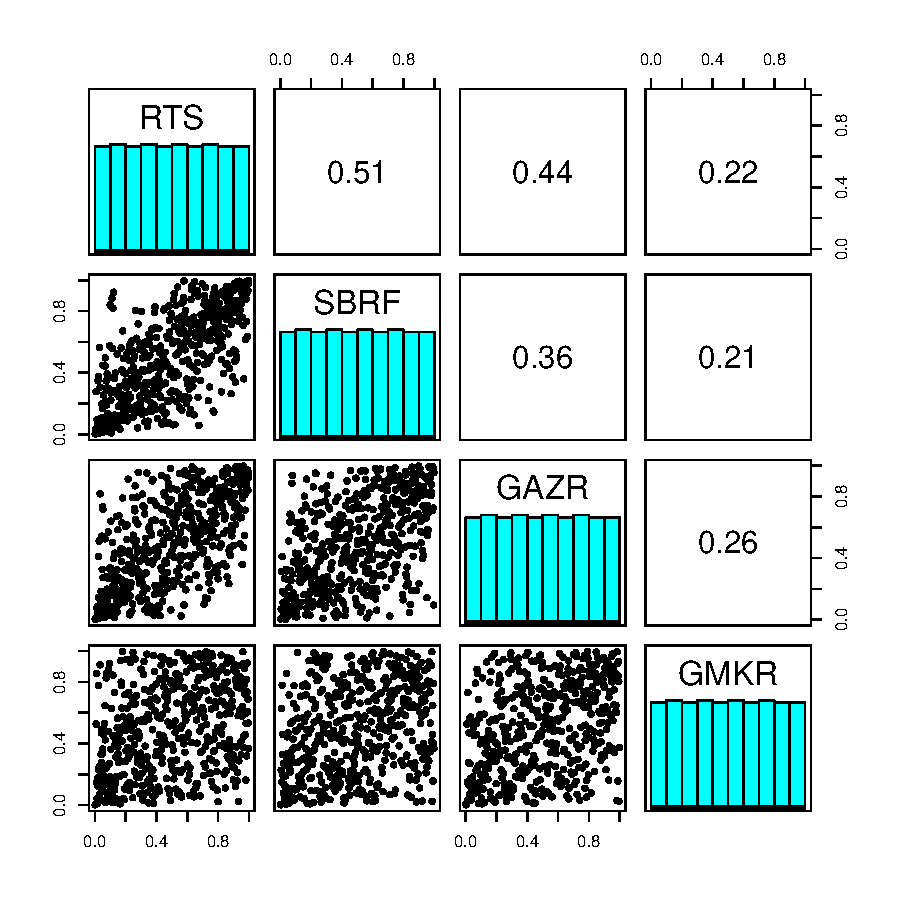
\includegraphics[width=0.49\textwidth]{PseudoObs.pdf}
  \caption{Парные графики наблюдений (слева) и псевдо-наблюдений (справа)}
  \label{ris:pobs}
\end{figure}

%\imgh[thb]{pobs.png}{width=\textwidth}{Парные графики наблюдений (слева) и псевдо-наблюдений (справа)}{pobs}

Операция преобразования лог-доходностей в псевдо-наблюдения описана уравнением~(\ref{pobs}).
Графики парных совместных распределений реальных наблюдений и полученных псевдо-наблюдений изображены на рис.~\ref{ris:pobs}.

Полученные псевдо-наблюдения далее используются для фитинга моделей копула согласно методологии, описанной в главе~\ref{methodology:copula}.
% Полученные результаты отображены в таблице~\ref{tab:copfit}.
Итогами фитинга модели Гауссовой копулы является корреляционная матрица, копулы Стьюдента -- корреляционная матрица и число степеней свободы. Их значения
%
\begin{equation} \label{gausscopfit}
    \Sigma_{Gauss} = \left(
    \begin{array}{cccc}
        1 & & & \\
        0.723 & 1 & & \\
        0.642 & 0.540 & 1 & \\
        0.335 & 0.320 & 0.391 & 1
    \end{array} \right),
\end{equation}

\begin{equation} \label{tcopfit}
    \Sigma_t = \left(
    \begin{array}{cccc}
        1 & & & \\
        0.723 & 1 & & \\
        0.642 & 0.540 & 1 & \\
        0.335 & 0.320 & 0.391 & 1
    \end{array} \right), \ \nu = 4.
\end{equation}

Как можно заметить, корреляционные матрицы для обеих копул идентичны. 
Это происходит потому, что оценка первого параметра многомерной копулы определяется только зависимостью между переменными.

Пусть каждому из активов \{RTS, SBRF, GAZR, GMKR\} портфеля соответствует ряд псевдо-наблюдений $u_i$, где $i$ -- порядковый номер актива, $i \in \overline{1,d}$. 
Тогда результаты фитинга вайн копулы можно описать следующей структурой:
%
\begin{enumerate}[(i)]
    \item Дерево 1:\\
    $c_{u_1;u_2}$ -- копула Стьюдента с параметрами $\rho=0.72$, $\nu=7.57$, $\tau=0.51$;\\
    $c_{u_3;u_1}$ -- копула Survival BB1 (повёрнутая на $180^{\circ}$ копула Клейтона-Гумбеля) с параметрами $\theta=0.12$, $\delta=1.68$, $\tau=0.44$;\\
    $c_{u_4;u_3}$ -- копула Survival Gumbel (повёрнутая на $180^{\circ}$ копула Гумбеля) с параметрами $\delta=1.33$, $\tau=0.25$;
    \item Дерево 2:\\
    $c_{u_3,u_2;u_1}$ -- копула Гумбеля с параметрами $\delta=1.1$, $\tau=0.09$;\\
    $c_{u_4,u_1;u_3}$ -- копула Клейтона с параметрами $\delta=0.16$, $\tau=0.07$;
    \item Дерево 3:\\
    $c_{u_4,u_2;u_3,u_1}$ -- копула Франка с параметрами $\delta=0.54$, $\tau=0.06$.
\end{enumerate}

Эта же структура может быть представлена в виде набора матриц $M$, $F$, $P_1$ и $P_2$, показанных в ур.~(\ref{vinefit}). 
Матрица $M$ определяет структуру дерева, остальные матрицы -- $F$, $P_1$ и $P_2$ -- указывают для каждого узла (парной копулы) набор семейств, первый и второй параметры соответственно. 
Если копула имеет только один параметр, то таковым является $\delta$, если же копула двух-параметрическая, то первым и вторым параметрами являются $\theta$ и $\delta$ соответственно.
В матрице $F$ введены сокращения для обозначения семейств: $St$ -- Стьюдента, $Gu$ -- Гумбеля, $Cl$ -- Клейтона, $Fr$ -- Франка, $SBB1$ -- Survival BB1, $SG$ -- Survival Gumbel.
%
\begin{gather} \label{vinefit}
    M = \left(
        \begin{array}{cccc}
        2 &   &   &   \\
        4 & 1 &   &   \\
        3 & 4 & 3 &   \\
        1 & 3 & 4 & 4 \\
        \end{array} \right), \ \
    F = \left(
        \begin{array}{lll}%{*4{C{5em}}}
        Fr\ &\  &    \\
        Gu\ &\ Cl\ &   \\
        St\ &\ SBB1\ &\ SG\
        \end{array} \right),\\    
    P_1 = \left(
        \begin{array}{ccc}
        0.544 & & \\
        1.098 & 0.158 & \\
        0.722 & 0.124 & 1.327
        \end{array} \right), \ \
    P_2 = \left(
        \begin{array}{ccc}
        0 &  & \\
        0 & 0 & \\
        7.566 & 1.682 & 0
        \end{array} \right). \nonumber
\end{gather}

% Тестирование ----
Результаты тестов полученных моделей показаны в таблице~\ref{tab:coptest}.
Для многомерных Гауссовой и Стьюдента копул был рассчитан функционал Крамера\,--\,фон~Мизеса, а для вайн копулы -- статистика Уайта.
Основываясь на значение $p$-value GoF-тестов оценки параметров, у нас нет основании отвергать нулевую гипотезу о принадлежности копул одному из распределений на 5\% уровне значимости.
Однако по их значениям для R-vine копулы можно заключить, что эта модель является наиболее адекватной из всех по отношению к реальным данным.

\begin{table}[h]
\centering
\caption{Оценка параметров копул и результаты тестирования}
\label{tab:coptest}
\setlength{\tabcolsep}{8pt}
\begin{tabular}{l|rr}
\hline
Копула & Статистика & $p$-value \\ \hline
Гауссова  & $S_n=0.034$ & 0.19 \\
Стьюдента & $S_n=0.391$ & 0.05 \\
R-vine    & $W=15.15$   & 0.95    \\ \hline
\end{tabular}
\end{table}

\subsection{Результаты оптимизации}
\label{calibration:optim}

В результате решения оптимизационной задачи (\ref{minES}) получили портфель со следующей структурой: $\textbf{w} = \{0.05, 0.114, 0.384, 0.452\}$. 
Здесь каждое значение -- это доля вложения активов RTS, SBRF, GAZR и GMKR соответственно.
Для того, чтобы убедиться в целесообразности выполнения оптимизации, я сравниваю риск метрики полученного портфеля со значениями, полученными для равновесного портфеля.
Для данного сравнения можно обойтись обычным историческим методом расчёта VaR и CVaR.
В качестве уровней задаются значения вероятностей $\pmb{\upalpha} = \{90\%, 95\%, 99\%, 99.5\%, 99.9\%\}$.

\begin{table}[h]
    \centering
    \setlength{\tabcolsep}{5pt}
    \begin{tabularx}{0.8\textwidth}
    % {c *{3}{|r@{\,/\,}l}} 
    {>{\setlength{\hsize}{\hsize}}Y 
    *{3}{|>{\setlength{\hsize}{\hsize}}R
    @{\ /\ }>{\setlength{\hsize}{\hsize}}X}}
    \hline
\multirow{2}{*}{$\upalpha$, \%} & \multicolumn{6}{c}{$\emph{VaR}_\alpha$ / $\emph{CVaR}_\alpha$, $\times 10^{-2}$} \\ \cline{2-7} 
& \multicolumn{2}{c|}{Оптимальный} & \multicolumn{2}{c|}{Равновесный} & \multicolumn{2}{c}{Смещение, $\times 10^{-2}$} \\ \hline
90\%   & $1.31$ & $2.01$ & $1.32$ & $2.14$ & $0.01$ & $0.13$ \\ 
95\%   & $1.69$ & $2.48$ & $1.82$ & $2.74$ & $0.13$ & $0.25$ \\ 
99\%   & $2.59$ & $3.96$ & $2.79$ & $4.36$ & $0.21$ & $0.41$ \\ 
99.5\% & $3.63$ & $5.22$ & $4.05$ & $5.50$ & $0.43$ & $0.28$ \\ 
99.9\% & $5.62$ & $5.86$ & $6.05$ & $6.29$ & $0.44$ & $0.43$ \\ 
\hline
    \end{tabularx}
    \caption{Сравнение равновесного и оптимального портфеля}
    \label{tab:eqw-optim}
\end{table}

В таблице~\ref{tab:eqw-optim} приведены риск метрики для обоих портфелей и пяти уровней. 
Четвёртая колонка в таблице показывает разницу между результатами, равную абсолютной разности риск метрик, полученных для равновесного и оптимального портфелей. 
При расчёте как VaR, так и CVaR для всех заданных уровней оптимальный портфель показал более консервативную оценку.
Это говорит о целесообразности выполнения оптимизации портфеля.